\documentclass{article}
\usepackage[utf8]{vietnam}
\usepackage[12pt]{extsizes}
\usepackage{amsmath,amsfonts,amsthm}
\usepackage{mathrsfs}
\usepackage{enumitem}
\usepackage{geometry}
\usepackage{mathtools}
\usepackage{booktabs}
\usepackage{pgfplots}
\usepackage{amssymb}
\usepackage{array}
\usepackage{multirow}
\usepackage{tabularx}
\usepackage{hyperref}
 \geometry{
 a4paper,
 total={170mm,257mm},
 left=20mm,
 top=20mm,
 }
 \usepackage{graphicx}
 \usepackage{titling}
 \usepackage{listings}
 \title{Lab 1: Lập trình Shell trên Linux
}
\author{23020874 Vũ Hàn Tín}
\date{Ngày 18/4/2025}
 \usepackage{fancyhdr}
\fancypagestyle{plain}{%  the preset of fancyhdr 
    \fancyhf{} % clear all header and footer fields
    \fancyfoot[L]{\thedate}
    \fancyhead[L]{ELT3296 Advanced Programming Techniques}
    \fancyhead[R]{\theauthor}
}
\makeatletter\def\@maketitle{%
\newpage
\null
\vskip 1em%
\begin{center}%
\let \footnote \thanks
  {\LARGE \@title \par}%
  \vskip 1em%
  %{\large \@date}%
\end{center}%
\par
\vskip 1em}
\makeatother
\begin{document}
\maketitle
\section{Lý thuyết}
\subsection{Khái niệm về Shell}
\begin{itemize}
    \item Shell là một giao diện CLI (Command Line Interface) hoạt động như một cầu nối tương tác giữa người dùng và kernel của hệ điều hành (Operating System).
    \item Shell cho phép người dùng thực hiện các tác vụ như quản lý file hay thực thi các chương trình,\dots
    \item Cấu trúc cơ bản của một câu lệnh Shell gồm 3 thành phần là:
    \begin{center}
    \begin{verbatim}
    command[options][arguments]
    \end{verbatim}
    \end{center}
    với \begin{itemize}
        \item \verb|command|: Câu lệnh trực tiếp được thực thi như ls, grep, \dots
        \item \verb|options|: Chỉnh sửa hành vi của câu lệnh, thường dùng với dấu $-$ hoặc $--$.
        \item \verb|arguments|: Xác định vị trí câu lệnh được thực thi ở đâu, như file hay directory.
        \end{itemize}
 \end{itemize}
 \subsection{Các câu lệnh Shell cơ bản}
 \subsubsection{Quản lý file và directory sử dụng Shell}
 File trong Linux được tổ chức theo dạng một tree với root là "/" cùng với các leaf tỏa ra xung quanh.
 \begin{figure}[h]
    \begin{center}
    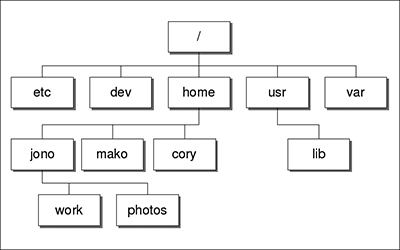
\includegraphics[width=10cm]{thfig04-09.jpg}
    \end{center}
    \end{figure} 
\\Có hai loại đường dẫn (path) là:
\begin{enumerate}
    \item Đường dẫn tuyệt đối (absolute path): là đường dẫn hoàn chỉnh của file hoặc directory, luôn bắt đầu từ "/", ví dụ như \verb|/home/Chiaki/LaTeX|.
    \item Đường dẫn tương đối (relative path): là đường dẫn đến directory đang làm việc hiện tại. Đường dẫn này không bắt đầu với "/" và sử dụng kí tự đặc biệt "." và ".." để chỉ directory hiện tại và parent của nó.\\ Ví dụ như để truy cập vào subdirectory \verb|LaTeX| từ \verb|~| ta gõ \verb|./LaTeX|.
\end{enumerate}
Trong Linux, chế độ truy cập file (file access mode) có thể quy định ai là người có quyền đọc (read), viết (write) hay thực thi (execute) file. Các chế độ này đều hiển thị qua câu lệnh \verb|ls -l|.
\\ Trong Linux cũng có 3 loại users được định nghĩa như sau:
\begin{itemize}
    \item Owner (user-u): Người tạo file.
    \item Group(g): Những người cùng nhóm với user.
    \item Others(o): Những người không cùng nhóm với user.
\end{itemize}
Các file hay directory trong Linux đều có 3 kiểu permissions:
\begin{center}
    \begin{tabular}{ | m{5em} | m{5cm}| m{5cm} | } 
      \hline
      Symbol & Permissions & Description \\ 
      \hline
      \verb|r| & Read & Can only view file content \\ 
      \hline
      \verb|w| & Write & Can modify or delete file \\ 
      \hline
      \verb|x|& Execute & Can run the file \\
      \hline
    \end{tabular}
    \end{center}
 Ví dụ, sau khi chạy lệnh \verb|ls -l| tại một directory, ta có kết quả sau:
 \begin{verbatim}
    -rw-r--r-- 1 Chiaki Chiaki  191637 Mar 11 21:56  signals_and_systems.pdf 
 \end{verbatim}
 Ta có thể thấy rằng chỉ có owner (Chiaki) mới có quyền được đọc và sửa file này (read and write), còn các user khác như group hay others đều chỉ có thể đọc (read) file.
 \\ Tổng hợp các câu lệnh cơ bản trong Shell cho quản lý file và directory:
 \begin{center}
    \begin{tabular}{ | m{5em} | m{7cm}| m{7cm} | } 
      \hline
      Command & Syntax & Description \\ 
      \hline
      \verb|pwd| & \verb|pwd| & Print current directory path \\ 
      \hline
      \verb|mkdir| & \verb|mkdir -p [directory]| & Create nested directory \\ 
      \hline
      \verb|chmod|& \verb|chmod [OPTIONS] MODE FILES | & Change user permission \\
      \hline
      \verb|cat| & \verb|cat > [file]| & Write a new file \\  
      
        & \verb|cat >> [file]|  & Append text to a file \\
      \hline
      \verb|echo| & \verb|echo "text"| & Print text to terminal \\  
      
        & \verb|echo "text" > [file]|  & Write text to a file \\
        & \verb|echo $VARIABLE|  & Print enviroment variable \\
      \hline
    \end{tabular}
    \end{center}
    \subsubsection{Quản lý tiến trình (process) với Shell}
    \begin{itemize}
        \item[-] Một tiến trình (process) trong Linux là biểu hiện của một chương trình đang hoạt động, tất cả các command hay application được thực thi trên Linux như là một tiến trình.
        \item[-] Các đặc tính của một tiến trình (process) gồm PID (process ID), PPID (parent process ID), UID (user ID), process state và CPU \& Memory usage. 
        \item[-] Câu lệnh \verb|ps -f| là câu lệnh dùng để hiển thị tất cả các đặc tính của tiến trình.
        \begin{verbatim}
        UID          PID    PPID  C STIME TTY          TIME CMD   
        Chiaki      7672    7665  0 08:21 pts/0    00:00:00 /bin/bash
        Chiaki     25971    7672  0 13:07 pts/0    00:00:00 ps -f
        \end{verbatim} 
        \item[-] Điều hướng tiến trình (redirecting process) là quá trình cho phép người dùng quản lý input, output và lỗi của các tiến trình.\\
        \begin{center}
        \begin{tabular}{ | l | l | l | }
            \hline
            Command & Description & Example usage \\ \hline            
            \verb|>| & Redirects stdout to a file (overwrites if exists) & \verb|ls > text.txt| \\ \hline      
            \verb|>>| & Redirects output to a file (appends only) & \verb|ps -f >> text.txt| \\ \hline      
            \verb|<| & Redirects input from a file instead of keyboard input & \verb|text.txt < cat| \\ \hline
            \verb|2>| & Redirects stderr to a file & \verb|ls error 2> error.log| \\ \hline
            \verb|2>>| & Appends errors message to a file & \verb|rm error 2>> error.log| \\ \hline
            \verb|&>| & Redirects stderr \& stdout to a file & \verb|ls error &> error.log| \\ \hline
          \end{tabular}
          \end{center}
    \end{itemize}
    \subsubsection{Interprocess communication in Linux (IPC)}
    \begin{itemize}
        \item IPC là phương thức cho phép nhiều tiến trình (process) chạy trên cùng một hệ thống có thể trao đổi dữ liệu và tín hiệu (data and signals) với các tiến trình khác.
        \item Pipe là một phương thức IPC đơn giản cho phép output của một tiến trình được sử dụng như input của một tiến trình khác. Pipe là phương thức chỉ cho dữ liệu đi theo một chiều (unidirectional).
        \item \verb|grep| là một câu lệnh được sử dụng để tìm kiếm text hoặc patterns trong các file. Cách sử dụng \verb|grep| như sau:
       \\ \begin{center}
        \begin{tabular}{| l | l | l|}
            \hline
            Command & Description \\
            \hline
            \verb|grep "pattern" file.txt|& Search for \verb|pattern| in file \\
            \hline
            \verb|grep -i "pattern" file.txt|& Case-insensitive search \verb|pattern| in file \\
            \hline
            \verb|grep -n "pattern" file.txt|& Show line numbers \\
            \hline
            \verb|grep -v "pattern" file.txt|& Show line not matching pattern \\
            \hline
            \verb|grep -w "pattern" file.txt|& Match whole word only \\
            \hline
            \verb|grep -c "pattern" file.txt|& Count occurences \\
            \hline
            \verb|grep -r "pattern" path|& Search recursively in directory \\
            \hline
        \end{tabular}
        \end{center}
        \item Một tín hiệu (signal) là một thông báo được gửi từ một tiến trình đến các tiến trình khác hay từ OS đến tiến trình.
       \\ \begin{center}
       \begin{tabular}{|l | l| l|}
          \hline
          Signals & Numbers & Description \\
          \hline
          SIGKILL & 9 & Immediately terminates a process (can't be ignored) \\
          \hline
          SIGTERM & 15 & Requests a process to kill terminate \\
          \hline
          SIGSTOP & 19 & Pauses a process \\
          \hline
          SIGCONT & 18   &Resumes a stopped process \\
          \hline
        \end{tabular}
      \end{center}
    \end{itemize}
    Ví dụ:
    \begin{center}
    \begin{verbatim}
      xournal & # open xournal
      ps -s | grep xournal
        6284 pts/0    00:00:00 xournal
      kill -9 6824
    \end{verbatim}
    \end{center}
\subsection{Giới thiệu về Shell script}
Có rất nhiều text editor có thể sử dụng để code Shell script như \verb|vim, nano, emacs|, nhưng ta chọn dùng \verb|vim| vì tính thuận tiện của nó.
Các bước để soạn Shell script bằng \verb|vim| như sau:
\begin{enumerate}
  \item Gõ câu lệnh \verb|vim| hoặc \verb|vim filename.sh| để truy cập vào \verb|vim|.
  \item \verb|vim| lúc này đang ở chế độ Normal mode, gõ \verb|i (insert)| hoặc \verb|a (append)|,
  \\ \verb|A(append from the end of line)| để truy cập vào Insert mode.
  \item Gõ file ở trong chế độ Insert mode và ấn phím esc để quay lại chế độ Normal mode.
  \item Chỉnh sửa file trong chế độ Normal mode và ấn \verb|:wq (write and quit)| để lưu file và thoát ra.
  \item Cấp quyền thực thi (execute) cho file trên terminal \verb|chmod u+x file.sh|.
  \item Thực thi file (execute) file \verb|./file.sh|.
\end{enumerate}
Tham khảo Vim cheatsheet để thao tác nhanh hơn trong Normal và Visual mode \url{https://devhints.io/vim}.
\subsection{Cấu trúc cơ bản của Shell script}
\subsubsection{Biến trong Shell}
Ta thường tạo ra biến trong Shell bằng cách sử dụng chúng (gán các giá trị khởi tạo) và truy cập thông qua toán tử
\verb|$|. Ngoài ra, ta có thể để cho người dùng nhập giá trị của biến đầu vào với câu lệnh \verb|read| và \verb|echo| để hiển thị giá trị của nó ra ngoài.
\\ Ví dụ: 
\\ \begin{verbatim}
  Chiaki@mx:~
$ variable=100
Chiaki@mx:~
$ echo $variable
100
Chiaki@mx:~
$ read X
123
Chiaki@mx:~
$ echo $X
123
\end{verbatim}
\subsubsection{Biến môi trường và biến tham số}
Khi khởi tạo Shell script, một số biến được khởi tạo giá trị từ môi trường (environment variables) và thường được viết
hoa toàn bộ (all uppercase) để phân biệt với các biến người dùng tự khởi tạo (user-defined) trong script, thường được viết chữ thường (lowercase).
\\ Ví dụ về các biến môi trường (environment variables) như: \verb|$HOME|, \verb|$USER|, \verb|$PWD|, \verb|$#| (number of parameters passed).
\subsubsection{Các lệnh so sánh trong Shell}
Các lệnh so sánh (conditions) được có thể chia làm 3 loại lớn gồm: so sánh chuỗi (string comparison), so sánh số học (arithmetics comparison) và file điều kiện (file conditional).
\\ Ngoài các phép so sánh cơ bản, Shell còn có các lệnh so sánh sau:
\begin{verbatim}
-n string1 (True if the string is not null)
-z string1 (True if the string is null)
expression1 (-eq, ne, gt, ge, lt, le) expression2
! expression (True if the expression is false)
-d file (True if the file is a directory)
-e file (True if the file exists)
-f file (True if the file is a regular file)
\end{verbatim}
\subsubsection{Các phép tính trong Shell}
Các phép tính trong Shell có cú pháp giống như trong các ngôn ngữ lập trình khác với các phép toán như \verb|+,-,*,/,%,=,| \dots, ví dụ:
\begin{verbatim}
  Chiaki@mx:~
$ X=100
Chiaki@mx:~
$ echo $(($X+3))
103
\end{verbatim}
\subsubsection{Cấu trúc điều khiển (control structure)}
Shell cũng có cấu trúc điều khiển giống với các ngôn ngữ lập trình khác với cú pháp như sau:
\begin{enumerate}
  \item If:
  \begin{verbatim}
    if conditions                 
      then 
        statements    
      else 
        statements
      fi
  \end{verbatim}
  \begin{verbatim}
#!/bin/sh
read x
if x % 2 -eq 0
    then echo "Even"
    else echo "Odd"
    fi
  \end{verbatim}
  \item While:
  \begin{verbatim}
    while condition 
    do
      statements
    done
  \end{verbatim}
  \begin{verbatim}
#!/bin/bash
x=1
while [ $x -le 5 ]
do
  echo "Welcome $x times"
  x=$(( $x + 1 ))
done
  \end{verbatim}
  \item For: 
  \begin{verbatim}
    for variables in values
      do statements
    done
  \end{verbatim}
  \begin{verbatim}
#!/bin/bash
for i in {1..5}
 do
     echo $i
done

  \end{verbatim}
  \item Until: Giống một phiên bản đảo ngược của While, khi mà câu lệnh được chạy cho tới khi nó \textbf{đúng} thì vòng lặp mới dừng.
  \begin{verbatim}
  until condition
    do
      statements
    done
  \end{verbatim}
  \begin{verbatim}
    #!/bin/bash
    x=1
    until [ $x -ge 5 ]
    do
      echo "Welcome $x times"
      x=$(( $x + 1 ))
    done
\end{verbatim}    
\end{enumerate}
\subsubsection{Hàm trong Shell}
Hàm (function) trong Shell cũng tương tự như hàm của các ngôn ngữ lập trình khác.
\begin{verbatim}
  function_name(){
    statements
  }

#!/bin/bash
add_two_num(){
    local sum=$(($1+$2))
    echo sum of $1 and $2 is $sum
}

add_two_num 2 3
\end{verbatim}
\section{Thực hành}
\subsection{Quản lý file và directory sử dụng Shell}
\subsubsection{Exercise 1:}
\begin{verbatim}
  Chiaki@mx:/                                                                                                                                                                                                    
  $ cd ~                                                                                                                                                                                                         
  Chiaki@mx:~                                                                                                                                                                                                    
  $ mkdir Slides Labs && touch Solution.txt                                                                                                                                                                      
  Chiaki@mx:~                                                                                                                                                                                                    
  $ cd ./Labs                                                                                                                                                                                                    
  Chiaki@mx:~/Labs                                                                                                                                                                                               
  $ mkdir Lab1 && touch Ex1.txt                                                                                                                                                                                  
  Chiaki@mx:~/Labs                                                                                                                                                                                               
  $ cp Ex1.txt ./Lab1                                                                                                                                                                                            
  Chiaki@mx:~/Labs                                                                                                                                                                                               
  $ rm -r Ex1.txt                                                                                                                                                                                                
  Chiaki@mx:~/Labs                                                                                                                                                                                               
  $ cd ./Lab1 && mv Ex1.txt Exercise1.txt                                                                                                                                                                        
  Chiaki@mx:~/Labs/Lab1                                                                                                                                                                                          
  $ chmod o+x Exercise1.txt                                                                                                                                                                                      
  Chiaki@mx:~/Labs/Lab1                                                                                                                                                                                          
  $ cd ~ && rm -r Slides
\end{verbatim}
\subsubsection{Exercise 2:}
\begin{verbatim}
  Chiaki@mx:~/Labs/Lab1                                                                                                                                                                                          
  $ cd                                                                                                                                                                                                           
  Chiaki@mx:~                                                                                                                                                                                                    
  $ pwd                                                                                                                                                                                                          
  /home/Chiaki
  Chiaki@mx:~                                                                                                                                                                                                    
  $ ls -al
  drwx------  4 Chiaki Chiaki  4096 Apr 10 23:36 .lgames                                                                                                                                                         
  drwxr-xr-x  6 Chiaki Chiaki  4096 Mar  7 20:41 .local                                                                                                                                                          
  drwx------  4 Chiaki Chiaki  4096 Mar  1 21:20 .mozilla 
  ...
  Chiaki@mx:~                                                                                                                                                                                                    
  $ cd .                                                                                                                                                                                                         
  Chiaki@mx:~                                                                                                                                                                                                    
  $ pwd                                                                                                                                                                                                          
  /home/Chiaki                                                                                                                                                                                                   
  Chiaki@mx:~                                                                                                                                                                                                    
  $ cd ..                                                                                                                                                                                                        
  Chiaki@mx:/home                                                                                                                                                                                                
  $ pwd                                                                                                                                                                                                          
  /home 
  Chiaki@mx:/home                                                                                                                                                                                                
  $ ls -al                                                                                                                                                                                                       
  total 12                                                                                                                                                                                                       
  drwxr-xr-x  3 root   root   4096 Feb 12 23:51 .                                                                                                                                                                
  drwxr-xr-x 19 root   root   4096 Apr 16 09:58 ..                                                                                                                                                               
  drwx------ 43 Chiaki Chiaki 4096 Apr 20 11:31 Chiaki                                                                                                                                                           
  Chiaki@mx:/home                                                                                                                                                                                                
  $ cd ..                                                                                                                                                                                                        
  Chiaki@mx:/                                                                                                                                                                                                    
  $ pwd                                                                                                                                                                                                          
  /     
  Chiaki@mx:/                                                                                                                                                                                                    
  $ ls -al                                                                                                                                                                                                       
  total 84                                                                                                                                                                                                       
  drwxr-xr-x  19 root root  4096 Apr 16 09:58 .                                                                                                                                                                  
  drwxr-xr-x  19 root root  4096 Apr 16 09:58 ..  
  ...       
\end{verbatim}
\subsubsection{Exercise 3:}
\begin{verbatim}
  Chiaki@mx:~/Labs/Lab1                                                                                                                                                                                          
  $ touch Hello.txt && echo "Hello..." > Hello.txt 
\end{verbatim}
Kết quả:
\begin{verbatim}
  Chiaki@mx:~/Labs/Lab1                                                                                                                                                                                          
  $ cat Hello.txt                                                                                                                                                                                                
  Hello everyone!                                                                                                                                                                                                
  This is Advanced Programming Techniques course.                                                                                                                                                                
  There are many exercises for you in this course.                                                                                                                                                               
  Let's practice what we learn in this course with exercises.                                                                                                                                                    
  Are you ready? 
\end{verbatim}
\subsubsection{Exercise 4:}
\begin{verbatim}
  Chiaki@mx:~/Labs/Lab1                                                                                                                                                                                          
  $ grep -c "course" Hello.txt > Ex4_results.txt 
  Chiaki@mx:~/Labs/Lab1                                                                                                                                                                                          
  $ sed -n "3p" "Hello.txt" | wc -w >> Ex4_results.txt 
  Chiaki@mx:~/Labs/Lab1                                                                                                                                                                                          
  $ cd ~ && ls -l >> ~/Labs/Lab1/Ex4_results.txt 
  Chiaki@mx:~                                                                                                                                                                                                    
  $ find -type f,d | wc -l >> ~/Labs/Lab1/Ex4_results.txt
  Chiaki@mx:~                                                                                                                                                                                                    
  $ find -type d | wc -l >> ~/Labs/Lab1/Ex4_results.txt 
  Chiaki@mx:~                                                                                                                                                                                                    
  $ ps -f | sed -n '$=' >> ~/Labs/Lab1/Ex4_results.txt                                                                                                                                                                                          
\end{verbatim}
\subsection{Shell script}
\subsubsection{Exercise 5:}
\begin{verbatim}
  #!/bin/sh
  # Name: Vu Han Tin, script name: greeting.sh, 
  # purpose of this script: practice shell script programming skill.
  echo "Hello + $USER" 
  neofetch
  id -g
  date
  cd ~ && ls
  echo "$TERM, $PATH, $HOME"
  timestamp=$(date)
  echo "Goodbye + $timestamp "
\end{verbatim}
\subsubsection{Exercise 6:}
\begin{verbatim}
  #!/bin/bash
  echo "Program name: $0"
  echo "Number of command line parameters: $#"
  echo "First command line parameter: $1"
  echo "All command line parameter:$@"
\end{verbatim}
\subsubsection{Exercise 7:}
\begin{verbatim}
  read decimal
  echo "obase=16;$decimal"| bc
\end{verbatim}
\subsubsection{Exercise 8:}
\begin{verbatim}
#!/bin/bash
fibonacci(){
    read input
    if((input <= 1))
        then echo 0
    elif((input == 2))
        then echo 1
    else
        n1=$((input-1))
        n2=$((input-2))
        a=$(echo $n1 | fibonacci)
        b=$(echo $n2 | fibonacci)
        echo $((a+b))
    fi
}
fibonacci
\end{verbatim}
\end{document}